\section{The First G-APD Cherenkov Telescope}

\begin{frame}{What is FACT?}
    \begin{columns}[T] % align columns
        \begin{column}{.45\textwidth}
            \vspace{10pt}
            \begin{itemize}
                \item "First G-APD Cherenkov Telescope"
                \item operating in la palma since 2011
                \item single telescope
                \item unis aufzählen?
                \item gapd's interessant für cta? wie genau? was ist das? wer nutzt das?
            \end{itemize}
        \end{column}
        \begin{column}{.48\textwidth}
            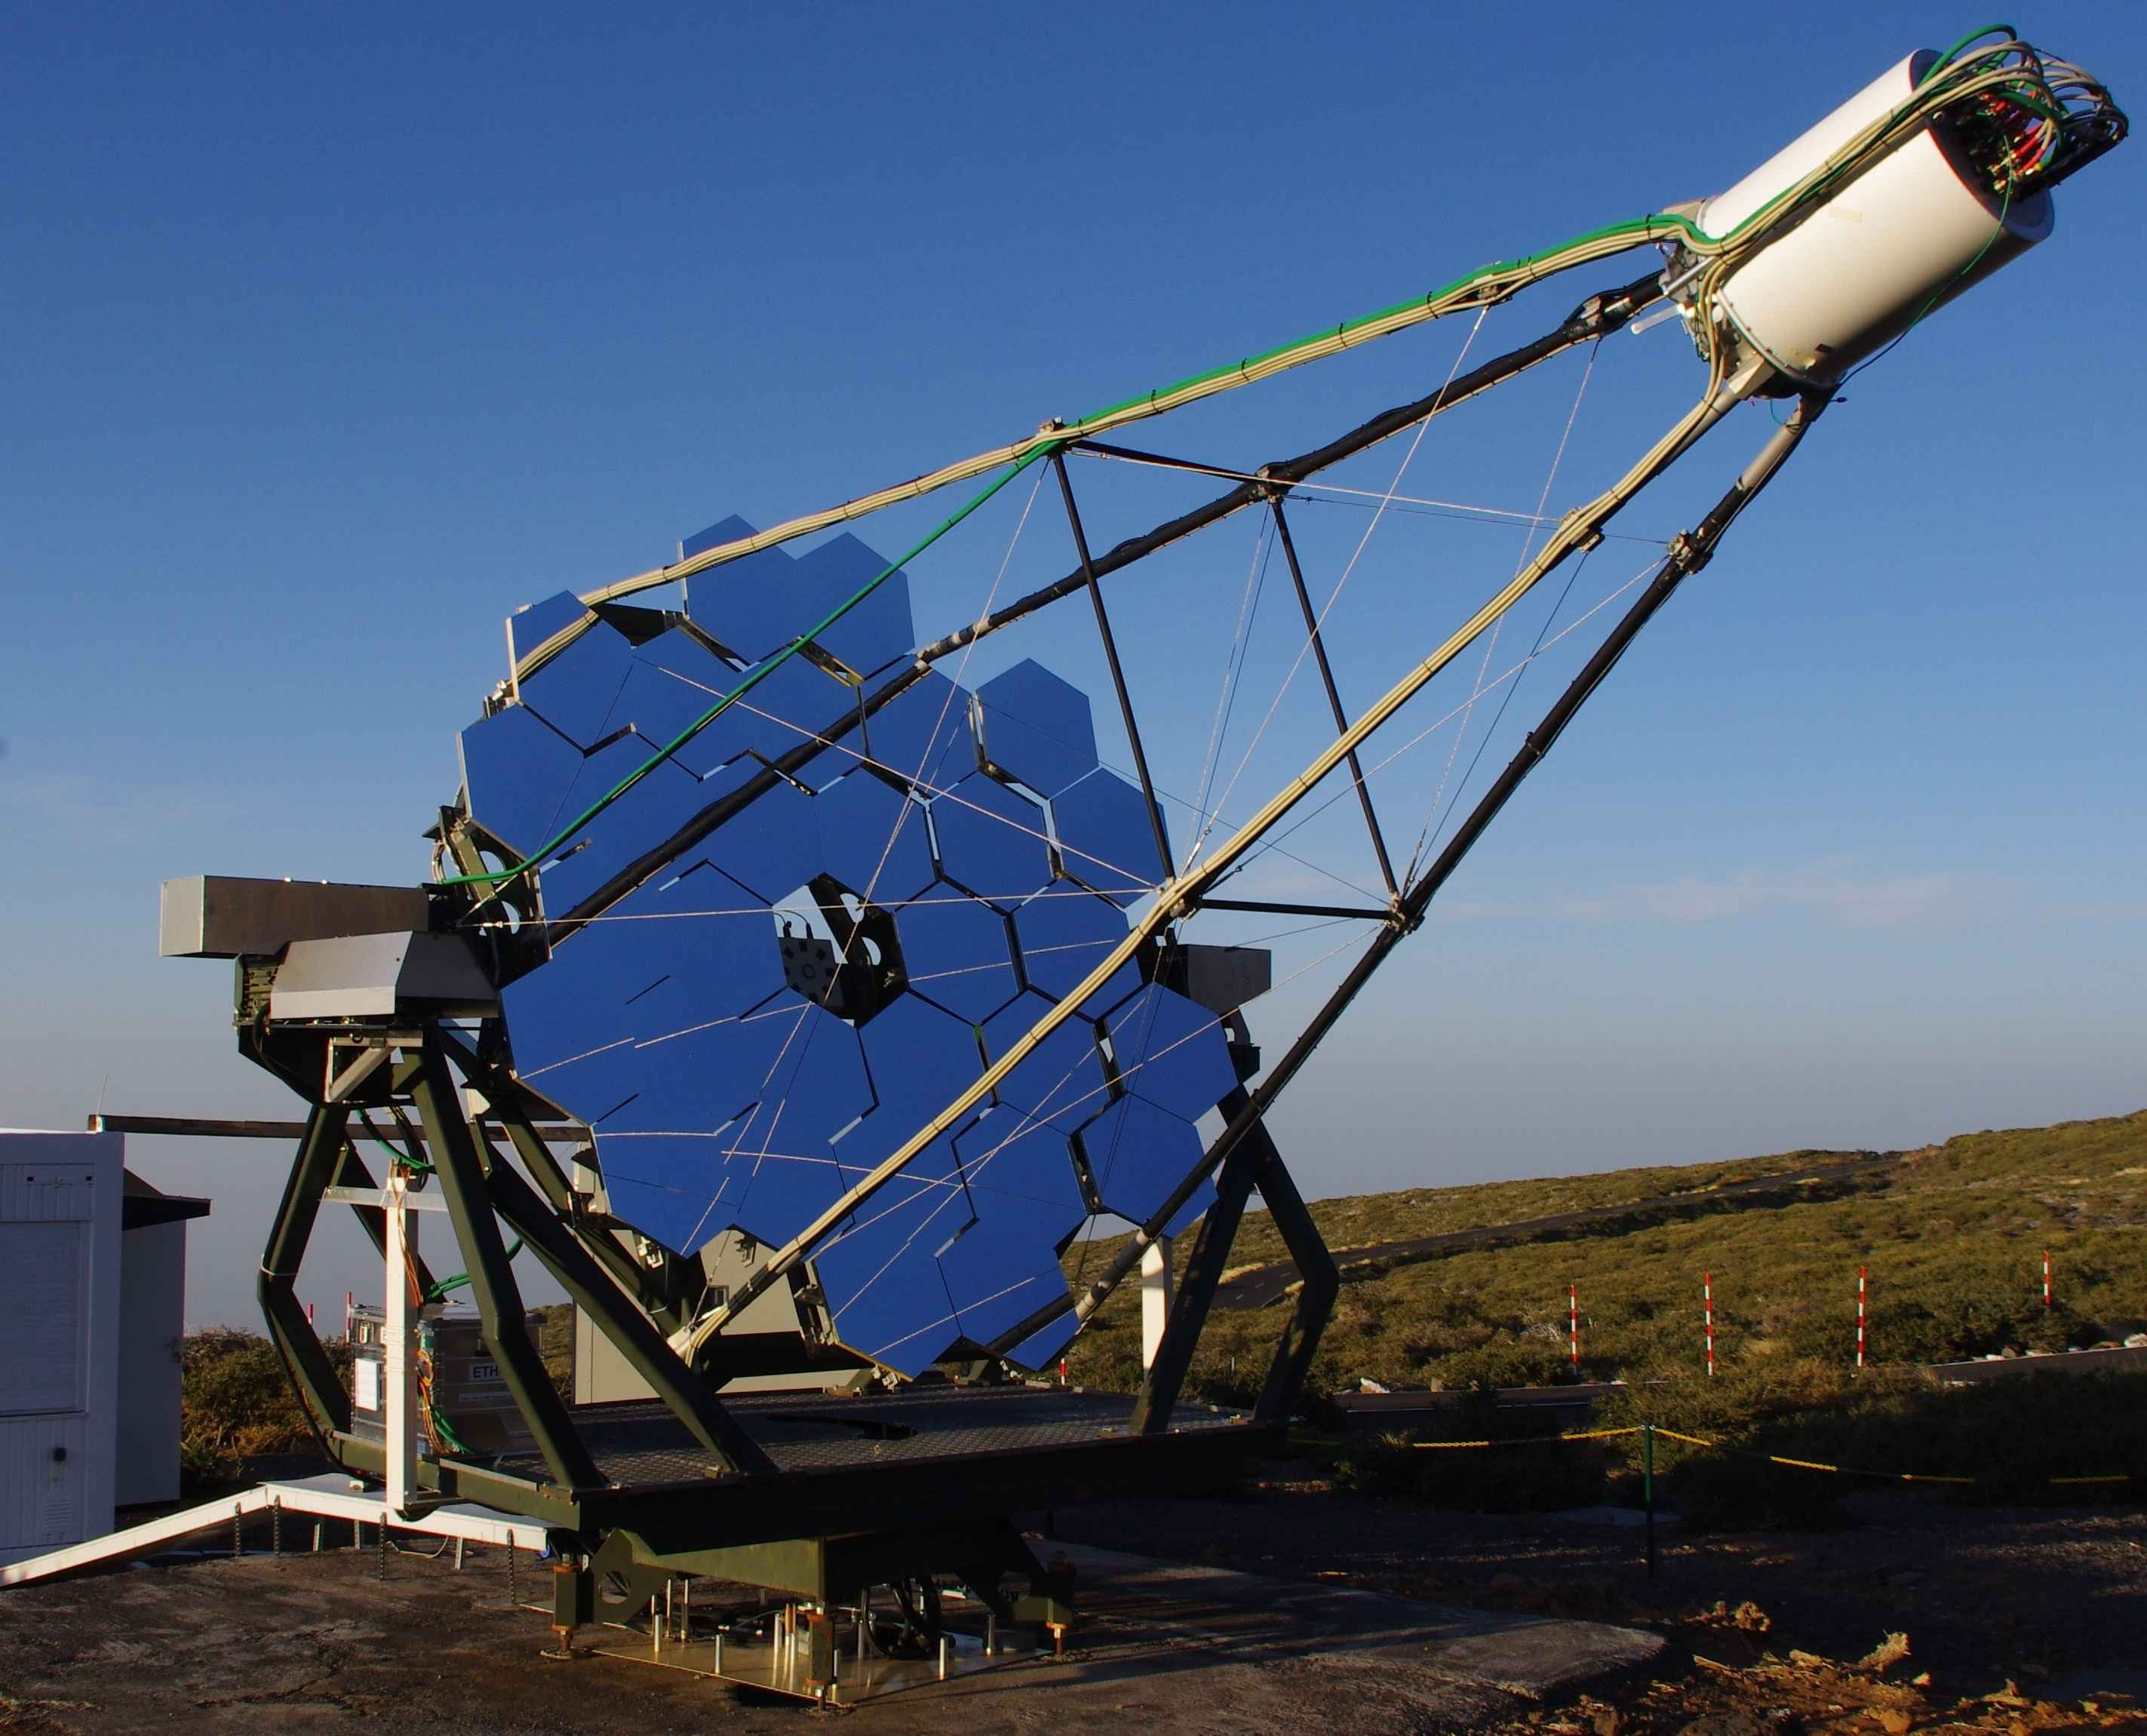
\includegraphics[width=\linewidth]{images/fact_telescope.jpg}
            \cite{Anderhub_2013}
        \end{column}
    \end{columns}
\end{frame}

\begin{frame}{Why does it matter?}
    \begin{enumerate}
        \item Knowledge in developing a processing pipeline 
        \item Single telescope analysis 
        \item Some features and methods might be useful for ctapipe
        \item e.g. cleaning based on arrival time
    \end{enumerate}
\end{frame}